%%%%%%%%%%%%%%%%%%%%%%%%%%%%%%%%%%%%%%%%%%%%%%%%%%%%%%%%%%%%%%%%%%%%%%%%%%%%%%%
% intro.tex: Introduction to the thesis
%%%%%%%%%%%%%%%%%%%%%%%%%%%%%%%%%%%%%%%%%%%%%%%%%%%%%%%%%%%%%%%%%%%%%%%%%%%%%%%%
\chapter{VLE model accelrated by ISAT}
\label{VLEISAT_chapter}
%%%%%%%%%%%%%%%%%%%%%%%%%%%%%%%%%%%%%%%%%%%%%%%%%%%%%%%%%%%%%%%%%%%%%%%%%%%%%%%%




\comment{
\section{Result and discussion} \label{sec:result}

We have integrated the aforementioned methods to develop an ISAT-VLE transcritical solver. In this section, we evaluate the performance and error control of the ISAT method through two sets of simulations: transcritical temporal mixing layer (Sec.~\ref{sec:TML}) and transcritical shock-droplet interaction (Sec.~\ref{sec:SD}). Both 3D and 2D settings are utilized for these simulations. The 2D simulations primarily serve as a means to test the ISAT method, as parallel computing introduces additional factors such as thread synchronization and inter-node communication, which can hinder an accurate assessment of ISAT's true performance. Furthermore, the 2D results can provide a suitable reference for determining the error tolerance in the 3D simulations. For the 3D configurations, we discuss the phase separation phenomena under transcritical conditions, along with demonstrating the tabulation error and ISAT performance. However, as mentioned earlier, the more complex parallel environment makes it challenging to measure the performance of a thermodynamic model in isolation. The 2D results serve as a more suitable reference for evaluation purposes.

Furthermore, in the transcritical shock-droplet interaction simulations (Sec.~\ref{sec:SD}), we compare the behavior of the double flux scheme (DF) and the fully conservative scheme (FC) with ISAT. Additionally, redundant record deletion methods are also evaluated in this Section.}

 %common part 

\section{Transcritical temporal mixing layer (TML)}
\subsection{3D TML ISAT simulations:}

As recommended in the preceding section, $k = 3\times 10^{-2}$ is used for the 3D TML simulation.
As suggested in the previous section, $k = 3\times 10^{-2}$ is used for the 3D TML simulations. Simulations of Case 1 and Case 2 are conducted with the configurations detailed in Table~\ref{TML_init_table}. A grid convergence study is conducted using the configuration of Case 1, shown in Appendix~\ref{App:TML}. The development of vortices is depicted in Fig.~\ref{TML_3D_evo}. At $t = 1\times 10^{-7}$, the introduction of velocity perturbation in the initial condition causes distortion of the interface. Due to the Kelvin-Helmholtz (K-H) instability, three vortices form on the interface at $1.5 \times 10^{-7}$. Within the vortex center, a low-pressure area is generated, and acoustic waves propagate outward continuously, which can be clearly seen in the pressure at $2\times 10^{-7}$. The quantity $\alpha=\beta(1-\beta)$ serves as an indicator of the two-phase interface. The $\alpha$ contours reveal that under these conditions, phase separation is highly pronounced at the interface between \ce{n-C12H26} and \ce{N2}.%, necessitating VLE modeling. 

\begin{figure}[htbp]
\centering
\includegraphics[width=0.65\linewidth]{TML_evo.png}
\caption{The vortex development in the 3D temporal mixing layer (TML): three snapshots at $t = 1\times 10^{-7}, 1.5 \times 10^{-7}, 2\times 10^{-7}$ s are shown in the figure.}
\label{TML_3D_evo} 
\end{figure}

Fig.~\ref{TML_3D_err} shows the temporal evolution of pressure and temperature errors. These values are obtained by calculating the absolute difference between the results obtained with the ISAT-VLE method and those obtained without it (e.g., $|T_{ISAT}-T_{noISAT}|$). As shown in Fig.~\ref{TML_3D_err}, both the temperature and pressure errors exhibit a gradual increase over time. However, the overall error remains at a very low level. The temperature deviation is primarily concentrated at the interface, with a maximum deviation of less than 5 K and a relative error of less than 1\%. The pressure error is more widespread due to the propagation of acoustic waves, but the majority of errors remain below 0.1 bar. The maximum error occurs at the interface and reaches approximately 0.2 bar. This error level is fully acceptable for the simulation, considering the average ambient pressure of around 50 bar, and the relative pressure error remains within 0.5\%.



\begin{figure}[htbp]
\centering
\includegraphics[width=0.65\linewidth]{TML_err.png}
\caption{The errors of the ISAT-VLE method in the 3D temporal mixing layer (TML): three snapshots at $t = 1\times 10^{-7}, 1.5 \times 10^{-7}, 2\times 10^{-7}$ s are shown in the figure.}
\label{TML_3D_err} 
\end{figure}


To compare the results of Case 1 and Case 2, a normalized time parameter $\tau = t \Delta U/ \delta_{\omega,0}$  is employed. Fig.~\ref{TML_3D_result} compares the results at $\tau = 45$, corresponding to the formation of the vortex. In both cases, a two-phase region is observed at the interface. However, in Case 2, the phase separation is significantly weaker despite the presence of cold \ce{N2} (293 K). This can be attributed to the high temperature of \ce{n-C12H26} (800 K), which hinders its cooling by the cold \ce{N2}.  As a result, even at the interface, the majority of mixtures remain in the gas phase. However, in the vicinity of the vortex, where mixing is more pronounced, a slightly stronger phase separation is observed. The crucial role of the VLE model becomes apparent in capturing these differences in phase separation under different conditions.


\begin{figure}[htbp]
\centering
\includegraphics[width=0.60\linewidth]{TML_2_cases2.png}

\caption{3D temporal mixing layer (TML) contours at $\tau = 45$ (in which $\tau = t \Delta U/ \delta_{\omega,0}$). Top (a,b): Case 1; Bottom (c,d): Case 2. Left (a,c): $\alpha$ (which is the indicator of the two-phase interface: $\alpha = \beta(1-\beta)$, where $\beta$ is vapor mole fraction); Right (b,d): mole fraction of \ce{n-C12H26}.}
\label{TML_3D_result} 
\end{figure}
The distinction between Case 1 and Case 2 can be better understood by analyzing through a phase diagram. Since the pressure variation in the TML simulation is relatively small, a temperature-mole fraction (T-X) diagram is employed to compare the two cases. In Fig.~\ref{TML_TX}, the phase boundaries at 50 bar and 40 bar serve as reference lines for the two-phase region. In Case 1, the lower initial temperature of \ce{n-C12H26} (600 K) causes the thermodynamic states of the mixing layer fluid ($X_{C_{12}H_{26}}$ within the range of 0.2-0.6) to overlap with the two-phase region, resulting in significant phase separation. However, in Case 2, the higher temperature of \ce{n-C12H26} (800 K) leads to points with $X_{C_{12}H_{26}}>0.3$ having temperatures above the two-phase boundary, thereby preventing phase separation in this region. Fig.~\ref{TML_TX} illustrates that the temperature of the phase boundary increases rapidly within the range of $X_{C_{12}H_{26}}<0.2$, making it difficult for the fluid in this region to remain outside the two-phase region in terms of thermodynamic properties. Consequently, Case 2 still exhibits weak phase separation. We further conducted tests with even higher initial \ce{n-C12H26} temperatures (up to 1200 K), resulting in further weakening of the phase separation, although it still persists.

\begin{figure}[htbp]
\centering
\includegraphics[width=0.45\linewidth]{TML_TX2.png}
\caption{The temperature-mole fraction (T-X) phase diagram of temporal mixing layer (TML) simulation: the phase boundary of \ce{N2}/\ce{C12H26} at 50 bar is shown in the plot as a solid black curve, and the region it encloses is the two-phase region at 50 bar.}
\label{TML_TX} 
\end{figure}

Fig.~\ref{TML_3D_performace} shows the performance of the ISAT-VLE method in the 3D simulation of Case 1. The simulation utilizes 128 CPU cores, and the CPU times presented in the figure represent the maximum time cost among all MPI processes at each time step. Initially, the ISAT-VLE method provides a speed-up of approximately 28 times. However, as the simulation progresses and more vortices form, the computational cost of ISAT-VLE increases. At the final time step, ISAT-VLE only achieves a speed-up of 1.5 times. This performance is very different from the one shown in Fig.~\ref{TML_PE}(a). The discrepancy arises because the ISAT-VLE method is more expensive in the interface region than the pure component region. This difference is attributable to the increased dispersion of thermodynamic states in the thermodynamic property space, necessitating more direct calculations of the VLE model. The distinct characteristics of different regions in the computational domain prevent the computing cores from synchronizing effectively. Consequently, the impact of data synchronization and communication between the computing cores becomes more pronounced, leading to longer waiting times. These challenges make it hard to accurately evaluate the performance of ISAT. Moreover, these issues are not solely related to the ISAT-VLE model but are also influenced by the overall CFD solver and hardware. Therefore, the 2D results provide a better reflection of the performance of ISAT-VLE.



\begin{figure}[htbp]
\centering
\includegraphics[width=0.45\linewidth]{time_p_TML_m.png}
\caption{Performance of the ISAT-VLE method in the 3D simulation of the temporal mixing layer (TML).}
\label{TML_3D_performace} 
\end{figure}

\comment{
    A grid convergence study is conducted using the configuration of Case 1, as shown in Appendix~\ref{App:TML}. The development of vortices is depicted in Fig.~\ref{TML_3D_evo}. At $t = 1\times 10^{-7}$ s, the introduction of velocity perturbation in the initial condition causes distortion of the interface. Due to the Kelvin-Helmholtz (K-H) instability, three vortices form on the interface at $1.5 \times 10^{-7}$ s. Within the vortex center, a low-pressure area is generated, and acoustic waves propagate outward continuously, which can be clearly seen in the pressure contours at $2\times 10^{-7}$ s. The quantity $\alpha=\beta(1-\beta)$ serves as an indicator of the two-phase interface and phase separation. The $\alpha$ contours reveal that at these conditions, phase separation is highly pronounced at the interface between \ce{n-C12H26} and \ce{N2}.%, necessitating VLE modeling. 


    \begin{figure}[htbp]
        \centering
        \includegraphics[width=0.65\linewidth]{TML_evo2.png}
        \caption{The vortex development in the 3D transcritical temporal mixing layer (TML): three snapshots at $t = 1\times 10^{-7}, 1.5 \times 10^{-7}, 2\times 10^{-7}$ s (from left to right) are shown in the figure.}
        \label{TML_3D_evo} 
        \end{figure}
        
        Fig.~\ref{TML_3D_err} shows the temporal evolution of pressure and temperature errors. These values are obtained by calculating the absolute difference between the results obtained with the ISAT-VLE method and those obtained without it (e.g., $|T_{ISAT}-T_{noISAT}|$). As shown in Fig.~\ref{TML_3D_err}, both the temperature and pressure errors exhibit a gradual and slow increase over time. However, the overall error remains at a very low level. The temperature deviation is primarily concentrated at the interface, with a maximum deviation of less than 5 K and a relative error of less than 1\%. The pressure error is more widespread due to the propagation of acoustic waves, but the majority of errors remain below 0.1 bar. The maximum error occurs at the interface and reaches approximately 0.2 bar. This error level is fully acceptable for the simulation, considering the average ambient pressure of around 50 bar, and the relative pressure error remains within 0.5\%.



}





\section{Transcritical shock-droplet interaction}
\subsection{Shock-droplet interaction in 3D simulations}
\label{sec:SD_3D}

In this subsection, we performed a series of 3D transcritical shock-droplet interaction simulations using the FC scheme. A grid convergence study is conducted, and results are shown in Appendix~\ref{App:SD}.Fig.~\ref{droplet_3d_1C} displays the 3D results at three different time instances: $5\times 10^{-7}$ s, $8.3\times 10^{-7}$ s, and $1.2\times 10^{-6}$ s, illustrating the propagation of the shock wave passing through the droplet. The results show the reflection wave and the deformation of the droplet induced by the shock wave. To gain a better understanding of the phase change, the thermodynamic state is plotted in the pressure-temperature (P-T) phase diagram (Fig.~\ref{droplet_3D_1C_phasediagram}). Since our focus is solely on the shock wave front and the interaction between the shock and droplet, data points corresponding to the expansion wave are excluded. In Fig.~\ref{droplet_3D_1C_phasediagram}, all data points can be clearly categorized into two distinct parts. The first part consists of points forming a curve in the lower right region, which represents the shock front connecting the pre-shock and post-shock ambient conditions. The second part comprises the remaining points, forming a band that corresponds to the droplet. This is attributed to the influence of \ce{n-C12H26}, causing the post-shock condition of the droplet to have lower pressure and temperature compared to the ambient post-shock condition. For the droplet points, the pressure undergoes a dramatic increase due to the shock wave, while the temperature remains relatively unchanged. A significant portion of these data points falls within the two-phase region (indicated by high $\alpha$ values), which requires VLE modeling. Moreover, despite the working pressure (350 bar - 400 bar) being much higher than the critical pressure of pure \ce{n-C12H26} (18 bar), the multi-component effect yields very high mixture critical pressures (560 bar at $x_N2 = 0.85$). As a result, the thermodynamic state is pushed back to the subcritical two-phase region (as depicted in Fig.~\ref{droplet_3D_1C_phasediagram}), leading to phase separation (as observed in Fig.~\ref{droplet_3d_1C}).

\begin{figure}[htbp]
\centering
\includegraphics[width=0.65\linewidth]{3D_shock_1C_2.png}
\caption{Transcritical shock-droplet interaction simulation with an initial temperature of 565 K: the top figures are density, and the bottom figures are $\alpha$, where $\alpha = \beta (1-\beta)$ is a two-phase interface indicator. From left to right are the time instants of $5\times 10^{-7}$ s, $8.3\times 10^{-7}$ s, and $1.2\times 10^{-6}$ s. }
\label{droplet_3d_1C} 
\end{figure}

\begin{figure}[htbp]
\centering
\includegraphics[width=0.50\linewidth]{PT_1C_2_p.png}
\caption{Phase diagram of the transcritical shock-droplet interaction simulation with an initial temperature 565 K. The label is the mole fraction of \ce{N2}. The data points are taken from the time instance of $1.2\times 10^{-6}$ s. The data points of the expansion wave are removed}
\label{droplet_3D_1C_phasediagram} 
\end{figure}

Fig.~\ref{SD_3D_err} illustrates the evolution of temperature and pressure errors in the 3D shock-droplet interaction simulation. It can be observed that these errors primarily manifest at the shock front and the acoustic waves generated by spurious oscillations. A notable distinction between the temperature and pressure errors is that the temperature error remains localized to the surface of the droplet, whereas the pressure error extends into the droplet's interior. This discrepancy arises due to the minimal influence of the shock wave on the droplet's temperature during its passage (as shown in Fig.~\ref{droplet_3d_1C}). Although the acoustic wave propagates the errors of both temperature and pressure over a wider region, their magnitudes are well-controlled. The temperature error is less than 0.1 K, and the pressure error remains below 0.2 bar. Both relative errors are maintained below 0.1\%. Consequently, the ISAT method demonstrates excellent error control in the 3D simulations.



\begin{figure}[htbp]
\centering
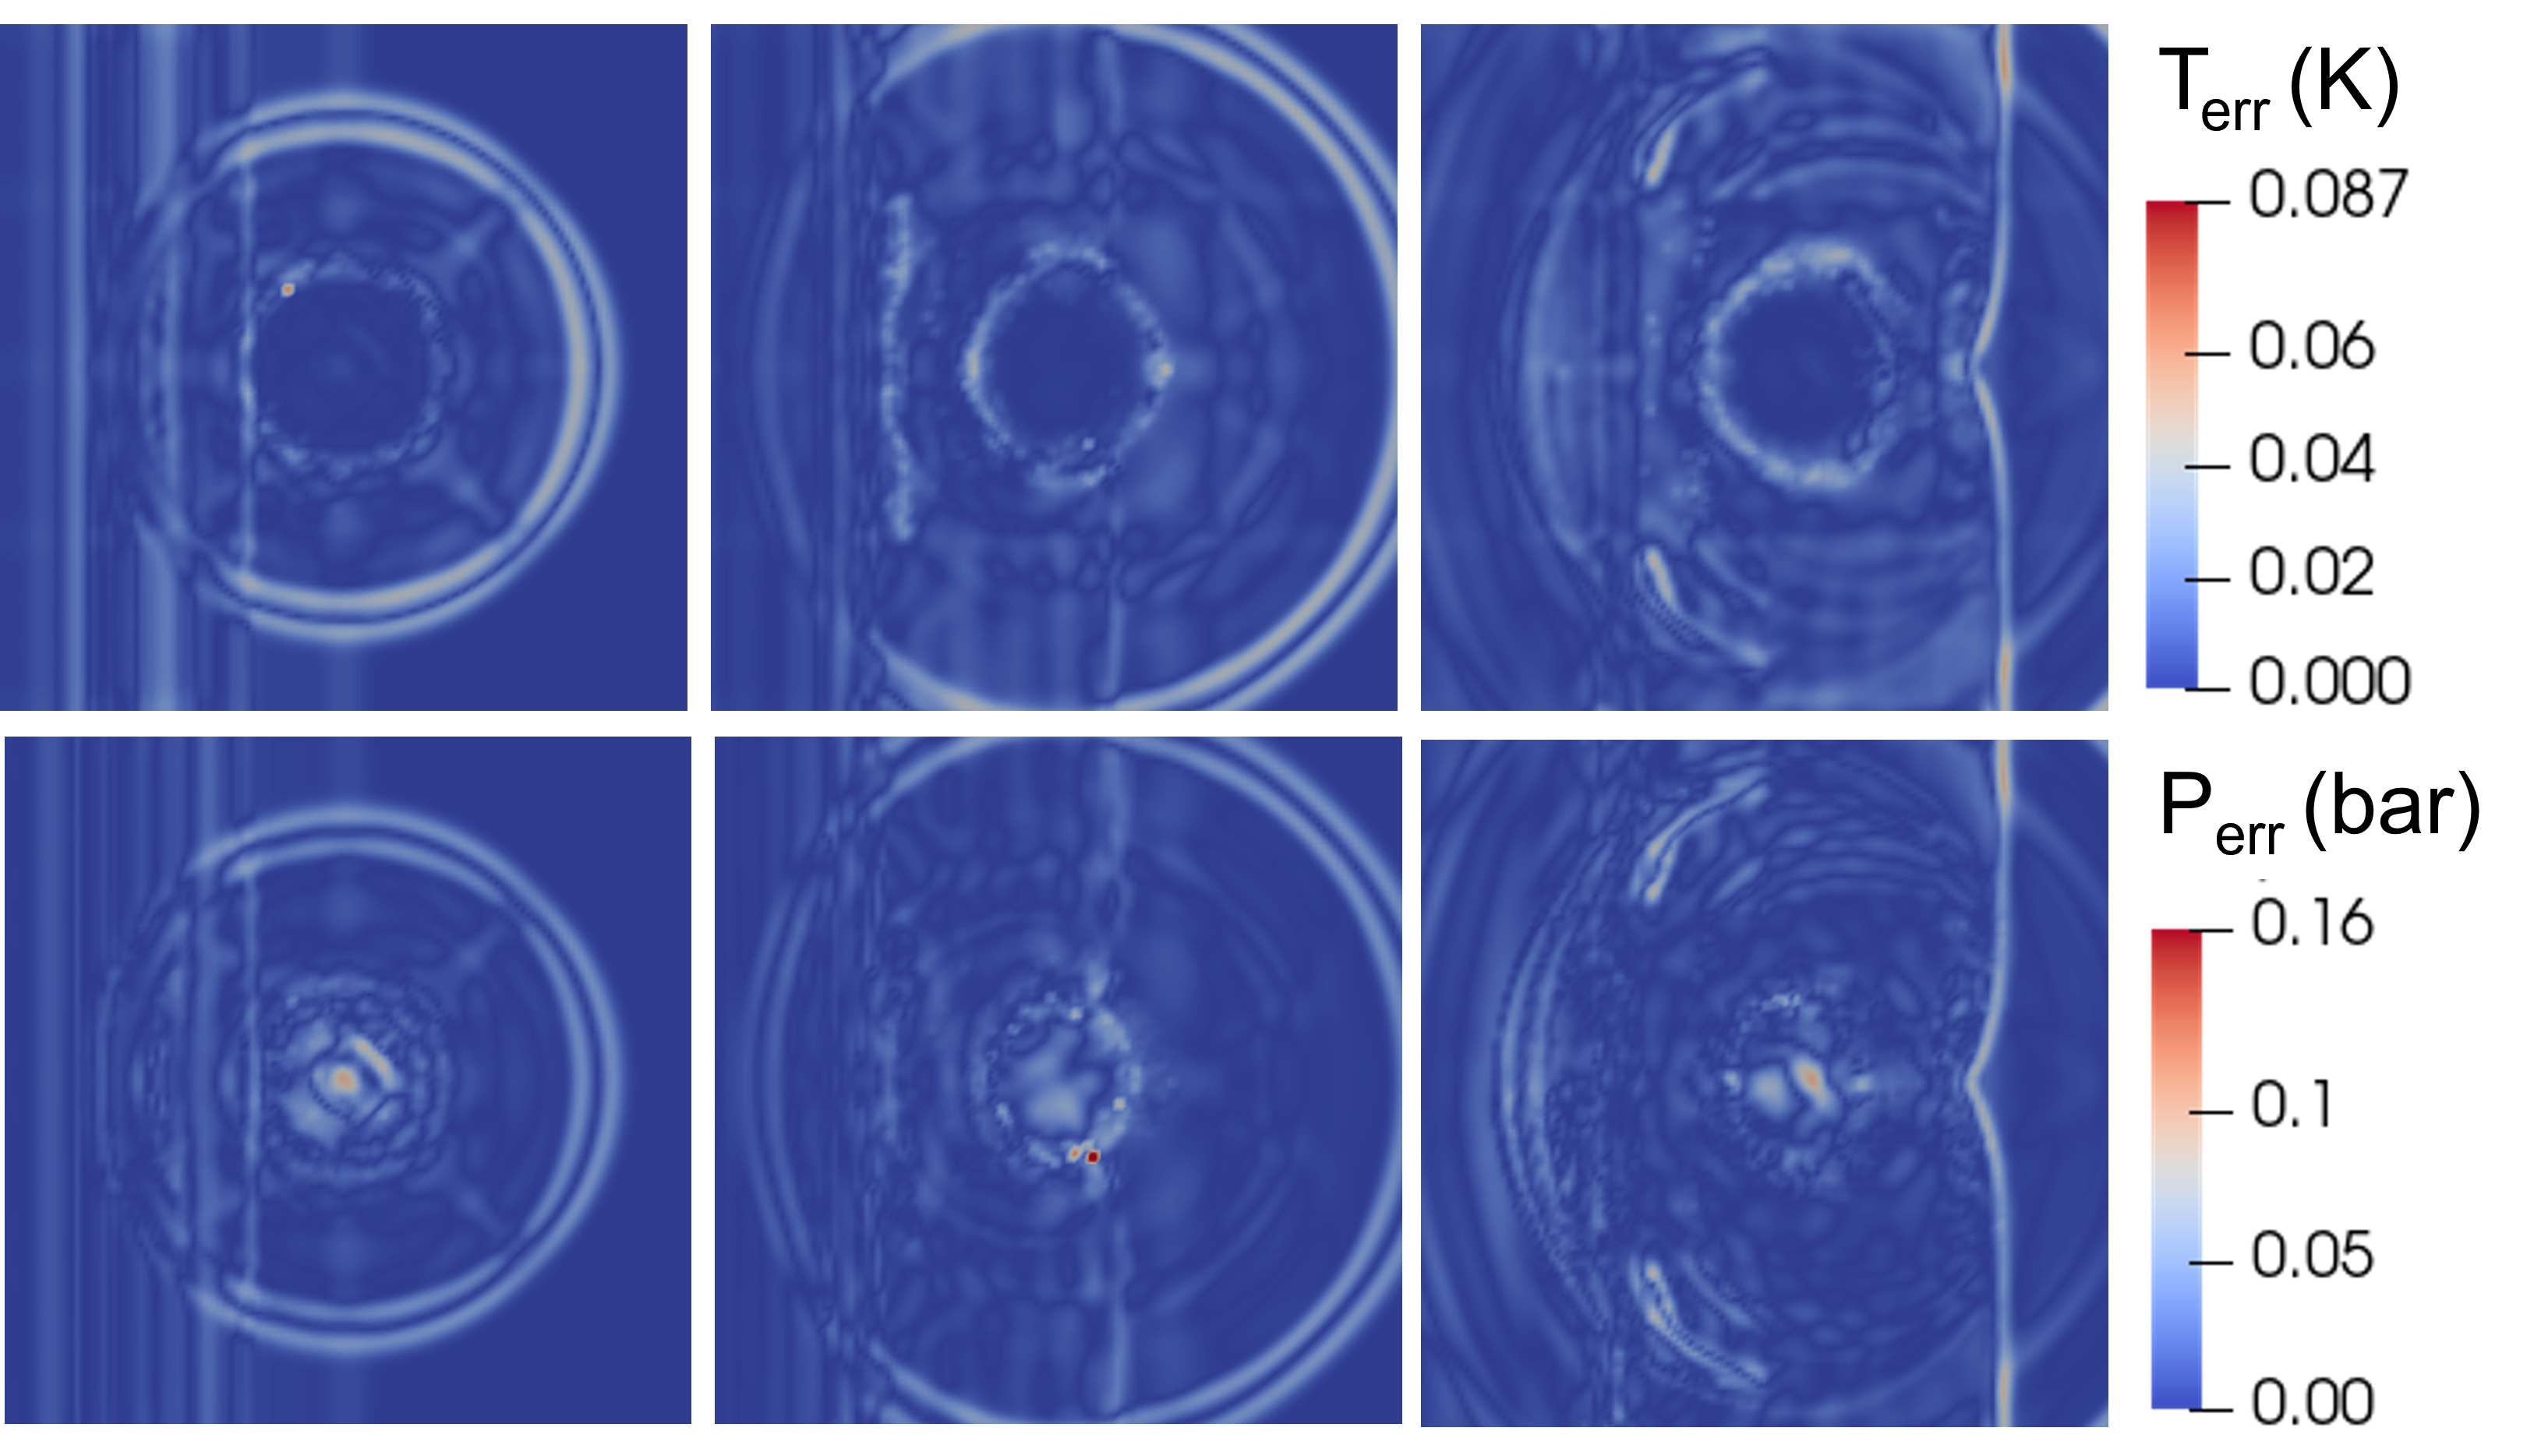
\includegraphics[width=0.65\linewidth]{3D_shock_1C_err_2.png}
\caption{The error contours of ISAT-VLE method in the 3D transcritical shock-droplet interaction simulation. From left to right are the time instants of $5\times 10^{-7}$ s, $8.3\times 10^{-7}$ s, $120\times 10^{-7}$ s. The labels in the figure are mole fractions.}
\label{SD_3D_err} 
\end{figure}

If the initial temperature is increased to 620 K, it significantly affects the phase separation effect at the interface. Initially, as shown in Fig.~\ref{droplet_3d_1C_HT}, the two-phase indicator $\alpha$ indicates that the droplet interface is situated within the subcritical two-phase region. However, as the shock wave passes through the droplet, the interface transitions into the single-phase region, eventually leading to the complete disappearance of the phase separation effect. This process is further illustrated in the phase diagram depicted in Fig.~\ref{droplet_3D_1C_HT_phasediagram}. The data points of the initial condition lie within the phase boundary of the mixture with $x_{N2}=0.7, x_{C12H26}=0.3$, confirming that the droplet interface exists in the subcritical two-phase region. As the shock wave elevates the droplet's pressure, the thermodynamic conditions move outside of the phase boundary, resulting in the elimination of phase separation. 

In this work, we did not include the modeling of surface tension. However, based on our findings, we anticipate that under these conditions, the mechanism of droplet break-up would be governed by surface tension prior to the shock wave, and subsequently influenced by the diffusion effect after the shock wave, as phase separation is eliminated.




\begin{figure}[htbp]
\centering
\includegraphics[width=0.65\linewidth]{3D_shock_1C_HT_3.png}
\caption{Transcritical shock-droplet interaction simulation with an initial temperature of 620 K: the top figures are density, the bottom figures are $\alpha$, where $\alpha = \beta (1-\beta)$ is a two-phase interface indicator. From left to right are the time instants of $5\times 10^{-7}$ s, $8.3\times 10^{-7}$ s, and $1.2\times 10^{-6}$ s.}
\label{droplet_3d_1C_HT} 
\end{figure}


\begin{figure}[htbp]
\centering
\includegraphics[width=0.50\linewidth]{PT_1C_HT_2_p.png}
\caption{Phase diagram of transcritical shock-droplet interaction simulation with an initial temperature 600K. Data points are taken from the time instance of $1.2\times 10^{-6}$ s. The labels in the figure are mole fractions.}
\label{droplet_3D_1C_HT_phasediagram} 
\end{figure}

Next, we explore the behavior of a two-component droplet. In this simulation, the droplet consists of 60\% \ce{n-C12H26} and 40\% \ce{n-C8H18} (by mole). The initial temperature is set to 565 K, which is consistent with the first case in this subsection. In Fig.~\ref{droplet_3d_2C}, as the shock wave passes through the droplet, we observe the disappearance of part of the two-phase boundary. This is because \ce{n-C8H18} has a lower critical temperature (\ce{n-C8H18} 568.9K, \ce{n-C12H26} 658.2 K) and changes the phase boundary (see in Fig.~\ref{droplet_3D_2C_phasediagram}) However, an additional phenomenon is also observed: even after the shock wave completely passes through the droplet, some sections of the droplet interface remain in the two-phase region. This is attributed to the relatively low pressure in the wake region behind the droplet, allowing the interface to remain in the subcritical two-phase region. This reasoning is clearly depicted in the phase diagram Fig.~\ref{droplet_3D_2C_phasediagram}, where the three-component system (\ce{n-C12H26}/\ce{n-C8H18}/\ce{N2}) exhibits a two-phase region overlapping with the low-pressure corner of the post-shock data points. Under such special conditions, the breakup of the droplet could be influenced by both surface effects and diffusion simultaneously, which could lead to the complex interaction of these mechanisms.





\begin{figure}[htbp]
\centering
\includegraphics[width=0.65\linewidth]{3D_shock_2C_2.png}
\caption{Transcritical shock-droplet interaction simulation with an initial temperature is 565K, and the droplet consists of 60\%\ce{n-C12H26} and 40\%\ce{n-C8H18} (by mole): the top figures are density, and the bottom figures are $\alpha$, where $\alpha = \beta (1-\beta)$ is a two-phase interface indicator. From left to right are the time instants of $5\times 10^{-7}$ s, $8.3\times 10^{-7}$ s, $120\times 10^{-7}$ s.}
\label{droplet_3d_2C} 
\end{figure}

\begin{figure}[htbp]
\centering
\includegraphics[width=0.50\linewidth]{TP_2C_2_p.png}
\caption{Phase diagram of transcritical shock-droplet interaction simulation with an initial temperature of 565K, and the droplet consists of 70\%\ce{n-C12H26} and 30\%\ce{n-C8H18} (by mass). Data points are taken from the time instance of $1.2\times 10^{-6}$ s. The labels in the figure are mole fractions.}
\label{droplet_3D_2C_phasediagram} 
\end{figure}

The 3D transcritical shock-droplet interaction simulations with a single-component droplet and an initial temperature of 565 K were conducted using 128 CPU cores. The performance of the ISAT-VLE method is illustrated in Fig.~\ref{droplet_3D_perf}. Initially, the ISAT-VLE case exhibited a speed-up of approximately 33 times compared to the VLE case without ISAT. Even in the later stages, it still maintained a significant speed-up of 15 times. On average, the ISAT-VLE method achieved a speed-up factor of approximately 17, showcasing its effectiveness in accelerating the simulations. Furthermore, it is evident that compared with the TML method (as shown in Fig.~\ref{TML_3D_performace}), the computational workload difference between different regions is not as pronounced, making the results closer to those obtained from 2D simulations.


 

\begin{figure}[htbp]
\centering
\includegraphics[width=0.5\linewidth]{time_parallel_new.png}
\caption{Performance of the ISAT-VLE method in the 3D transcritical shock-droplet interaction simulation.}
\label{droplet_3D_perf} 
\end{figure}



%%%%%%%%%%%%%%%%%%%%%%%%%%%%%%%%%%%%%%%%%%%%%%%%%%%%%%%%%%%%%%%%%%%%%%%%%%%%%%%%
